\chapter{霧裡看物理—擺}
\chapterauthor{張智閎}

\setcounter{section}{-1}
\section{前言}
Hi各位,我是熊熊,因為兔兔很懶不想打講義,所以叫編這本講義的熊熊隨便打一打,每個主題幫他留一頁空白就好,然後還給熊熊這些不合理的要求。
\begin{figure}[H]
\centering
\graphicspath{{physics/}}
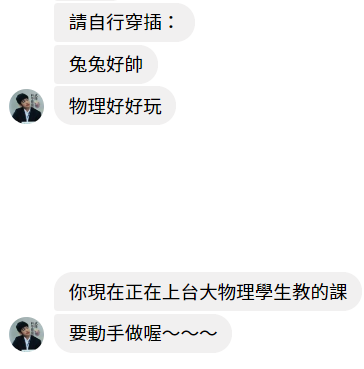
\includegraphics[width=7.5cm, center]{request.png}
\caption{不合理的要求} \vskip 10 pt
\label{fig:request}
\end{figure}
\newpage

\section{什麼是物理}
\newpage
\section{你該知道的事}
\newpage
\section{場?}
\newpage
\section{擺-1}
\newpage
\section{擺-2}
\newpage
\section{擺-3}
\newpage
\section{然後呢?}
\newpage

\newpage
\section{講師介紹}
\begin{itemize}
\item 姓名:張智閎
\item 性別:男
\item 特色:全班公認最電,高一去參加物奧選訓即獲得前半,保送台大物理(編按:本人表示自己不會念物理系)、偏矮,且從國小就如此、擔任圖資時,從不做事、幾乎所有自然科都免修,然後用免修的時間準備英文辯論或外交小尖兵,可謂不務正業的代表(編按:柏丞曰:「智閎感覺下學期不太認真耶」)、曾在緬甸與志工團隊同房睡時,講了整晚夢話,其中包括「草莓給我拿來」(編按:對講師大喊「草莓給我拿來」有機率獲得額外加成)。
\item 名言:我要看一下這題((寫,喔解出來、熊熊$\sim\sim\sim\sim$、熊熊你在幹嘛、草莓給我拿來。
\end{itemize}